\chapter{Barèmes}
\label{annexe:baremes}

L'équation suivante donne une équation exponentielle où la droite passe nécessairement par (0,1) et ($a$,0). Le ratio $a/b$ peut être ajusté pour donner la forme voulue à la courbe.
\begin{equation}
    y(x) = \frac{1-10^{\frac{x-a}{b}}}{1-10^{a/b}}
    \label{annexe:bareme_exp_poisson}
\end{equation}

\begin{figure}[h]
    \centering
    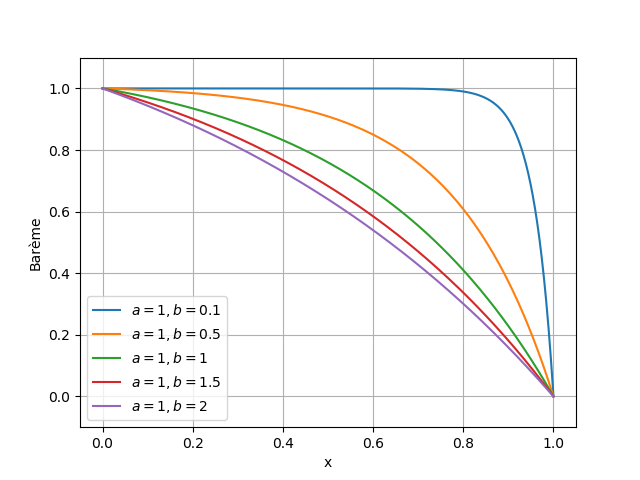
\includegraphics[width=0.75\linewidth]{fig/exp_poisson.png}
    \caption{Barème exponentielle pour la taille des poissons}
    \label{fig:exp_poisson}
\end{figure}